% Options for packages loaded elsewhere
\PassOptionsToPackage{unicode}{hyperref}
\PassOptionsToPackage{hyphens}{url}
%
\documentclass[
]{article}
\usepackage{amsmath,amssymb}
\usepackage{lmodern}
\usepackage{iftex}
\ifPDFTeX
  \usepackage[T1]{fontenc}
  \usepackage[utf8]{inputenc}
  \usepackage{textcomp} % provide euro and other symbols
\else % if luatex or xetex
  \usepackage{unicode-math}
  \defaultfontfeatures{Scale=MatchLowercase}
  \defaultfontfeatures[\rmfamily]{Ligatures=TeX,Scale=1}
\fi
% Use upquote if available, for straight quotes in verbatim environments
\IfFileExists{upquote.sty}{\usepackage{upquote}}{}
\IfFileExists{microtype.sty}{% use microtype if available
  \usepackage[]{microtype}
  \UseMicrotypeSet[protrusion]{basicmath} % disable protrusion for tt fonts
}{}
\makeatletter
\@ifundefined{KOMAClassName}{% if non-KOMA class
  \IfFileExists{parskip.sty}{%
    \usepackage{parskip}
  }{% else
    \setlength{\parindent}{0pt}
    \setlength{\parskip}{6pt plus 2pt minus 1pt}}
}{% if KOMA class
  \KOMAoptions{parskip=half}}
\makeatother
\usepackage{xcolor}
\IfFileExists{xurl.sty}{\usepackage{xurl}}{} % add URL line breaks if available
\IfFileExists{bookmark.sty}{\usepackage{bookmark}}{\usepackage{hyperref}}
\hypersetup{
  pdftitle={Laboratorio 04},
  hidelinks,
  pdfcreator={LaTeX via pandoc}}
\urlstyle{same} % disable monospaced font for URLs
\usepackage{longtable,booktabs,array}
\usepackage{calc} % for calculating minipage widths
% Correct order of tables after \paragraph or \subparagraph
\usepackage{etoolbox}
\makeatletter
\patchcmd\longtable{\par}{\if@noskipsec\mbox{}\fi\par}{}{}
\makeatother
% Allow footnotes in longtable head/foot
\IfFileExists{footnotehyper.sty}{\usepackage{footnotehyper}}{\usepackage{footnote}}
\makesavenoteenv{longtable}
\usepackage{graphicx}
\makeatletter
\def\maxwidth{\ifdim\Gin@nat@width>\linewidth\linewidth\else\Gin@nat@width\fi}
\def\maxheight{\ifdim\Gin@nat@height>\textheight\textheight\else\Gin@nat@height\fi}
\makeatother
% Scale images if necessary, so that they will not overflow the page
% margins by default, and it is still possible to overwrite the defaults
% using explicit options in \includegraphics[width, height, ...]{}
\setkeys{Gin}{width=\maxwidth,height=\maxheight,keepaspectratio}
% Set default figure placement to htbp
\makeatletter
\def\fps@figure{htbp}
\makeatother
\setlength{\emergencystretch}{3em} % prevent overfull lines
\providecommand{\tightlist}{%
  \setlength{\itemsep}{0pt}\setlength{\parskip}{0pt}}
\setcounter{secnumdepth}{-\maxdimen} % remove section numbering
\ifLuaTeX
  \usepackage{selnolig}  % disable illegal ligatures
\fi

\title{Laboratorio 04}
\author{}
\date{}

\begin{document}
\maketitle

\hypertarget{tema-python}{%
\section{Tema: Python}\label{tema-python}}

\begin{longtable}[]{@{}
  >{\raggedright\arraybackslash}p{(\columnwidth - 4\tabcolsep) * \real{0.3290}}
  >{\raggedright\arraybackslash}p{(\columnwidth - 4\tabcolsep) * \real{0.3355}}
  >{\raggedright\arraybackslash}p{(\columnwidth - 4\tabcolsep) * \real{0.3355}}@{}}
\toprule
\begin{minipage}[b]{\linewidth}\raggedright
\begin{quote}
\textbf{Estudiante}
\end{quote}
\end{minipage} & \begin{minipage}[b]{\linewidth}\raggedright
\begin{quote}
\textbf{Escuela}
\end{quote}
\end{minipage} & \begin{minipage}[b]{\linewidth}\raggedright
\begin{quote}
\textbf{Asignatura}
\end{quote}
\end{minipage} \\
\midrule
\endhead
\begin{minipage}[t]{\linewidth}\raggedright
\begin{quote}
Juan José Condori Pinto

Jcondoripin@unsa.edu.pe
\end{quote}
\end{minipage} & \begin{minipage}[t]{\linewidth}\raggedright
\begin{quote}
Escuela Profesional de

Ingenier´ıa de Sistemas
\end{quote}
\end{minipage} & \begin{minipage}[t]{\linewidth}\raggedright
\begin{quote}
Programaci´on Web 2
\end{quote}
\end{minipage} \\
\bottomrule
\end{longtable}

\begin{longtable}[]{@{}
  >{\raggedright\arraybackslash}p{(\columnwidth - 4\tabcolsep) * \real{0.3290}}
  >{\raggedright\arraybackslash}p{(\columnwidth - 4\tabcolsep) * \real{0.3355}}
  >{\raggedright\arraybackslash}p{(\columnwidth - 4\tabcolsep) * \real{0.3355}}@{}}
\toprule
\begin{minipage}[b]{\linewidth}\raggedright
\begin{quote}
\textbf{Laboratorio}
\end{quote}
\end{minipage} & \begin{minipage}[b]{\linewidth}\raggedright
\begin{quote}
\textbf{Tema}
\end{quote}
\end{minipage} & \begin{minipage}[b]{\linewidth}\raggedright
\begin{quote}
\textbf{Duraci´on}
\end{quote}
\end{minipage} \\
\midrule
\endhead
\begin{minipage}[t]{\linewidth}\raggedright
\begin{quote}
04
\end{quote}
\end{minipage} & \begin{minipage}[t]{\linewidth}\raggedright
\begin{quote}
Python
\end{quote}
\end{minipage} & \begin{minipage}[t]{\linewidth}\raggedright
\begin{quote}
04 horas
\end{quote}
\end{minipage} \\
\bottomrule
\end{longtable}

\begin{longtable}[]{@{}
  >{\raggedright\arraybackslash}p{(\columnwidth - 4\tabcolsep) * \real{0.3290}}
  >{\raggedright\arraybackslash}p{(\columnwidth - 4\tabcolsep) * \real{0.3355}}
  >{\raggedright\arraybackslash}p{(\columnwidth - 4\tabcolsep) * \real{0.3355}}@{}}
\toprule
\begin{minipage}[b]{\linewidth}\raggedright
\begin{quote}
\textbf{Semestre acad´emico}
\end{quote}
\end{minipage} & \begin{minipage}[b]{\linewidth}\raggedright
\begin{quote}
\textbf{Fecha de inicio}
\end{quote}
\end{minipage} & \begin{minipage}[b]{\linewidth}\raggedright
\begin{quote}
\textbf{Fecha de entrega}
\end{quote}
\end{minipage} \\
\midrule
\endhead
\begin{minipage}[t]{\linewidth}\raggedright
\begin{quote}
2023 - A
\end{quote}
\end{minipage} & \begin{minipage}[t]{\linewidth}\raggedright
\begin{quote}
29 Mayo 2023
\end{quote}
\end{minipage} & \begin{minipage}[t]{\linewidth}\raggedright
\begin{quote}
09 Junio 2023
\end{quote}
\end{minipage} \\
\bottomrule
\end{longtable}

\begin{enumerate}
\def\labelenumi{\arabic{enumi}.}
\item
  \begin{quote}
  \textbf{Competencias del curso}
  \end{quote}
\end{enumerate}

\begin{quote}
General: C.c. Disen˜a responsablemente aplicaciones web, sus componentes
o procesos para sa- tisfacer necesidades dentro de restricciones
realistas: econ´omicas, medio ambientales, sociales, pol´ıticas,
´eticas, de salud, de seguridad, manufacturaci´on y sostenibilidad.

Espec´ıfica: C.m. Construye responsablemente soluciones con tecnolog´ıa
web siguiendo un proceso adecuado llevando a cabo las pruebas ajustada a
los recursos disponibles del cliente.

Espec´ıfica: C.p. Aplica de forma flexible t´ecnicas, m´etodos,
principios, normas, est´andares y herramientas del desarrollo web
necesarias para la construcci´on de aplicaciones web e implemen- taci´on
de estos sistemas en una organizaci´on.
\end{quote}

\hypertarget{resultado-del-estudiante}{%
\section{Resultado del estudiante}\label{resultado-del-estudiante}}

\begin{quote}
RE. 2: La capacidad de aplicar disen˜o de ingenier´ıa para producir
soluciones a problemas y disen˜ar sistemas, componentes o procesos para
satisfacer necesidades espec´ıficas dentro de con- sideraciones
realistas en los aspectos de salud pu´blica, seguridad y bienestar;
factores globales, culturales, sociales, econ´omicos y ambientales.

RE. 8: La capacidad de crear, seleccionar y utilizar t´ecnicas,
habilidades, recursos y herramientas modernas de ingenier´ıa y
tecnolog´ıas de la informaci´on, incluyendo la predicci´on y el modela-
miento, con una comprensi´on de las limitaciones.
\end{quote}

\hypertarget{equipos-materiales-y-temas}{%
\section{Equipos, materiales y temas}\label{equipos-materiales-y-temas}}

\begin{quote}
Sistema Operativo (GNU/Linux de preferencia). GNU Vim.

Python 3. Git.

Cuenta en GitHub con el correo institucional. Entorno virtual.
\end{quote}

\hypertarget{tarea}{%
\section{\texorpdfstring{Tarea }{Tarea }}\label{tarea}}

\begin{quote}
URL GitHub de Tarea del Ajedrez (Repositorio individual)
\end{quote}

\begin{quote}
Estos objetos estarán disponibles importando la biblioteca:
\textbf{chessPictures} y estar´an interna- mente representados con
arreglos de \textbf{strings} que podr´a revisar en el archivo
\textbf{pieces.py}

La clase \textbf{Picture} tiene un s´olo atributo: el arreglo de strings
\textbf{img}, el cual contendr´a la represen- taci´on en caracteres de
la figura que se desea dibujar.

La clase \textbf{Picture} ya cuenta con una funci´on implementada, no
debe modificarla, pero si puede usarla para implementar sus otras
funciones:

\textbf{invColor:} recibe un color como un caracter de texto y devuelve
su color negativo, tambi´en como texto, deber´a revisar el archivo
\textbf{colors.py} para conocer los valores negativos de cada caracter.

La clase \textbf{Picture} contar´a adem´as con varios m´etodos que usted
deber´a implementar:
\end{quote}

\begin{itemize}
\item
  \textbf{verticalMirror:} Devuelve el espejo vertical de la imagen
\end{itemize}

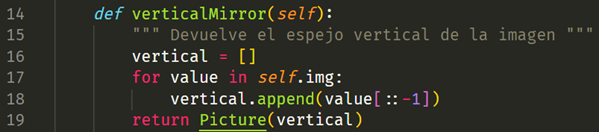
\includegraphics[width=6.23928in,height=1.37528in]{media/image4.png}

La función utiliza la siguiente lógica: si la figura espejo vertical de
una imagen es representada de forma invertida o reflejada,eso significa
que para cada fila de su estructura los caracteres están invertidos o
simplemente la columna está ordenada inversamente, por tal motivo la
función recorre la imagen y añade a una nueva lista cada línea de texto
de forma invertida, esto mediante el operador ::-1 dentro de los
corchetes de cada valor.

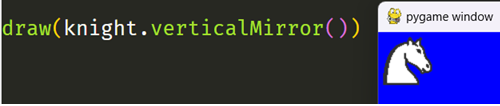
\includegraphics[width=5.23379in,height=1.08343in]{media/image5.png}

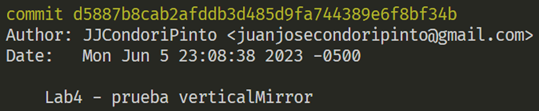
\includegraphics[width=5.61715in,height=1.15843in]{media/image6.png}

Commit de implementación y prueba del método verticalMirror()

\begin{itemize}
\item
  \textbf{horizontalMirror:} Devuelve el espejo horizontal de la imagen
\end{itemize}

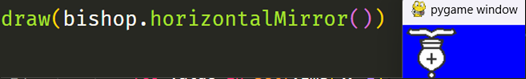
\includegraphics[width=6.33929in,height=1.37025in]{media/image7.png}

Siguiendo la misma lógica que en el anterior método, si queremos ver la
imagen de forma invertida o reflejada horizontalmente, ya no será
necesario recorrer cada línea de texto de manera inversa, sino que ir
imprimiendo la figura de abajo hacia arriba, es decir, de forma
invertida, es por ello que ahora se itera con la lista de imagen
invertida.

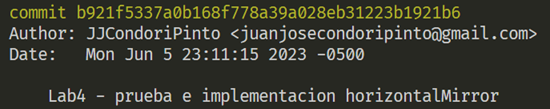
\includegraphics[width=5.46458in,height=0.80972in]{media/image8.png}

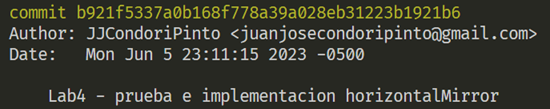
\includegraphics[width=5.7255in,height=1.13343in]{media/image9.png}

Commit de prueba e implementación del método horizontalMirror()

\begin{itemize}
\item
  \textbf{negative:} Devuelve un negativo de la imagen
\end{itemize}

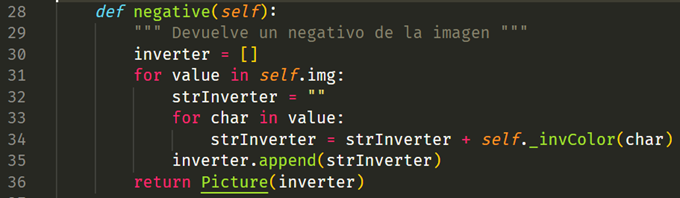
\includegraphics[width=7.08333in,height=2.06042in]{media/image10.png}

El método negative devuelve la imagen con los colores invertidos, por
tal motivo ahora necesitamos iterar sobre cada carácter de la lista, en
ese sentido ya tenemos un método que permite extraer el color invertido
de un carácter, solo lo concatenamos en una línea entera y esa la
indexamos a nuestra nueva imagen.

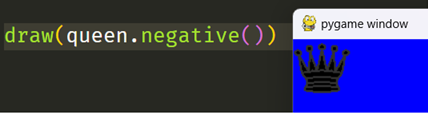
\includegraphics[width=4.46458in,height=1.20208in]{media/image11.png}

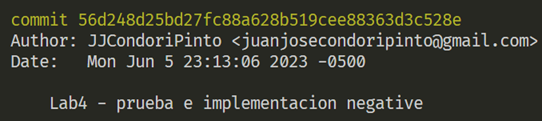
\includegraphics[width=5.65049in,height=1.25844in]{media/image12.png}

Commit de prueba e implementación del método negative()

\begin{itemize}
\item
  \textbf{join:} Devuelve una nueva figura poniendo la figura del
  argumento al lado derecho de la figura actual
\end{itemize}

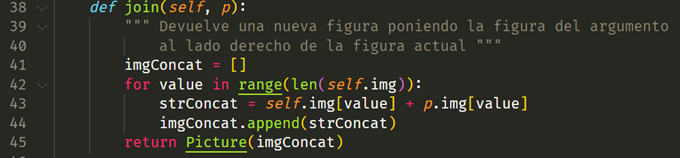
\includegraphics[width=7.08333in,height=1.65in]{media/image13.png}

Este método lo único que hace es concatenar cada línea de la imagen de
la figura con las líneas de la imagen de la figura a unir, es por ello
que el bucle itera sobre las posiciones de cada fila de la imagen, para
así concatenar las filas en dicha posición y añadirlo a una nueva
imagen.

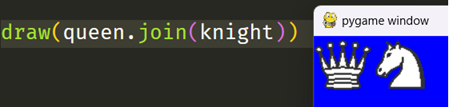
\includegraphics[width=4.67847in,height=1.11875in]{media/image14.png}

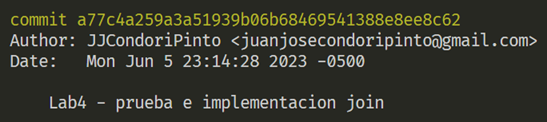
\includegraphics[width=5.70049in,height=1.27511in]{media/image15.png}

Commit de prueba e implementación del método join()

\begin{itemize}
\item
  \textbf{up:} Devuelve una nueva figura poniendo la figura recibida
  como argumento, encima de la figura actual
\end{itemize}

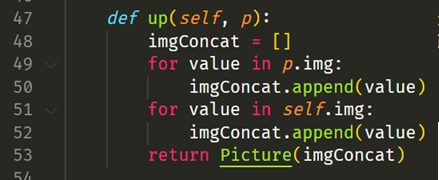
\includegraphics[width=4.56706in,height=1.87516in]{media/image16.png}

Este método recibe como parámetro a una figura, la lógica es la
siguiente: si queremos que una imagen esté dentro de otra, entonces
primero debemos imprimir la imagen de la primera figura y debajo la 2da,
es por ello que se realizan dos bucles, el primero para añadir la imagen
de la figura y el segundo para colocar por debajo a la 2da.

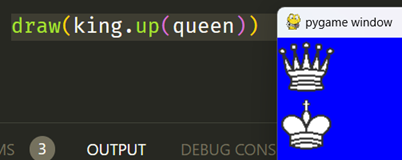
\includegraphics[width=4.19028in,height=1.66667in]{media/image17.png}

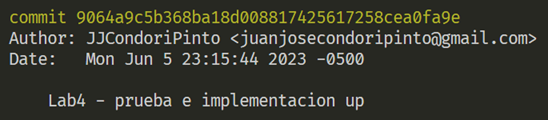
\includegraphics[width=5.70883in,height=1.25011in]{media/image18.png}

Commit de prueba e implementación del método up()

\begin{itemize}
\item
  \textbf{under:} Devuelve una nueva figura poniendo la figura recibida
  como argumento, sobre la figura actual
\end{itemize}

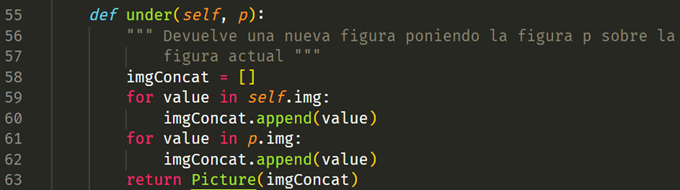
\includegraphics[width=7.08333in,height=1.97569in]{media/image19.png}

Este método utiliza la misma lógica del anterior, es decir, si ahora
queremos que la figura pasada como parámetro esté por debajo, entonces
la imprimimos al final, por lo cual, primero debemos añadir a la figura
actual y seguido la 2da, a la inversa.

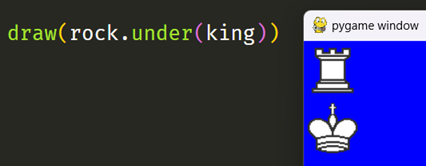
\includegraphics[width=4.44028in,height=1.72639in]{media/image20.png}

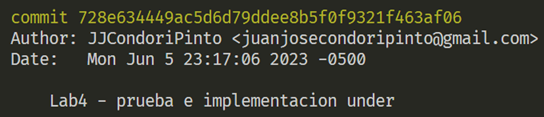
\includegraphics[width=5.66716in,height=1.21677in]{media/image21.png}

Commit de prueba e implementación del método under()

\begin{itemize}
\item
  \textbf{horizontalRepeat:} Devuelve una nueva figura repitiendo la
  figura actual al costado la cantidad de veces que indique el valor de
  n
\end{itemize}

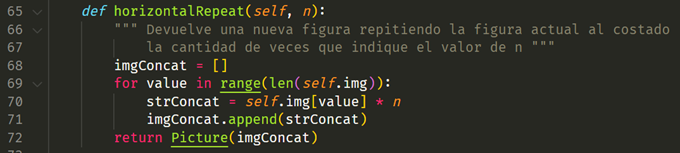
\includegraphics[width=7.08333in,height=1.59583in]{media/image22.png}

Para este método, si queremos que la imagen se repita n veces de forma
horizontal, entonces debemos de repetir n veces cada fila de la imagen,
por lo cual, iteramos en cada fila de dicha imagen y guardamos en una
nueva lista cada línea multiplicada n veces la repetición que pasemos
como parámetro.

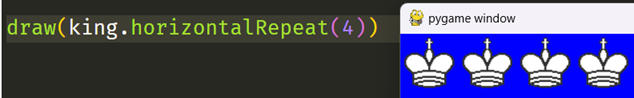
\includegraphics[width=6.60139in,height=1.01806in]{media/image23.png}

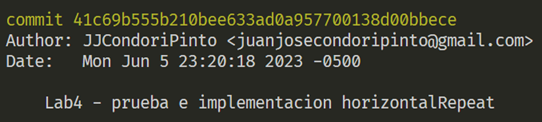
\includegraphics[width=5.65049in,height=1.27511in]{media/image24.png}

Commit de prueba e implementación del método horizontalRepeat()

\begin{itemize}
\item
  \textbf{verticalRepeat:} Devuelve una nueva figura repitiendo la
  figura actual debajo, la cantidad de veces que indique el valor de n
\end{itemize}

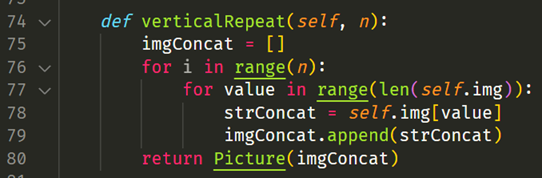
\includegraphics[width=5.65049in,height=1.85016in]{media/image25.png}

Para este método seguimos la misma lógica que under(), ya que si
queremos que la figura se repita n veces una debajo de la otra, entonces
debemos de iterar n veces sobre dicha figura para que aparezca n veces
debajo de la misma, esto se generaliza en un bucle tal y como se ve en
la figura.

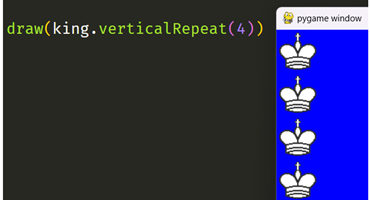
\includegraphics[width=3.85714in,height=2.0833in]{media/image26.png}

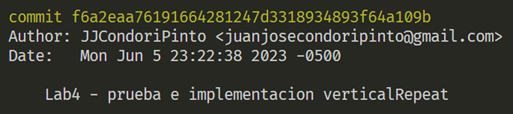
\includegraphics[width=5.33929in,height=1.19257in]{media/image27.png}

Commit de prueba e implementación del método verticalRepeat()

\begin{itemize}
\item
  \textbf{rotate:} Este método rota la imagen (de forma horaria o
  antihoraria) 90 grados
\end{itemize}

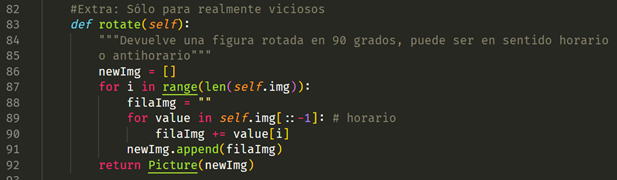
\includegraphics[width=6.42857in,height=1.88004in]{media/image28.png}

Este método se guía sobre la siguiente lógica: si tenemos una matriz y
queremos rotarla 90 grados, será necesario rotar tanto filas como
columnas en tal sentido, es decir, cambiar posiciones, es por ello que
este método itera sobre cada columna de la imagen y la va concatenando
desde el final (para girar de forma horaria), luego de ello se inserta
en una nueva lista como fila, al final dichas filas conforman una nueva
imagen rotada.

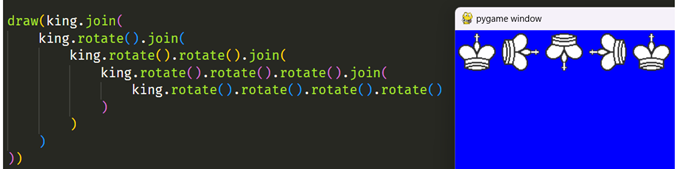
\includegraphics[width=7.07708in,height=1.75625in]{media/image29.png}

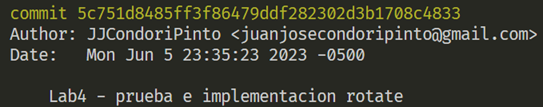
\includegraphics[width=5.65882in,height=1.1501in]{media/image30.png}

Commit de prueba e implementación del método rotate()

\begin{itemize}
\item
  \textbf{replace:} Este método inserta en los caracteres vacíos o
  espacios parte de la figura pasada como parámetro, es útil para
  insertar figuras en casillas o cuadros del tablero.
\end{itemize}

\begin{quote}
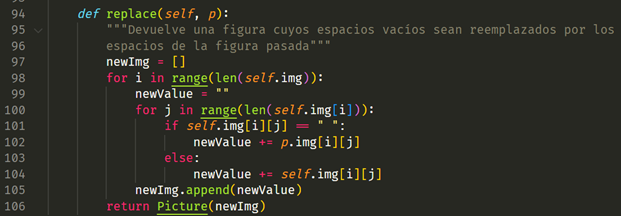
\includegraphics[width=6.46429in,height=2.24856in]{media/image31.png}

Este método recorre cada carácter de la imagen, si en caso uno de estos
sea un espacio vacío, se reemplaza con el carácter de la figura pasada
como parámetro, es por ello que se requieren dos índices, caso
contrario, se mantiene el espacio de la figura inicial.

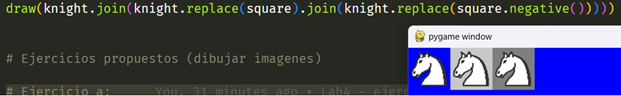
\includegraphics[width=6.46389in,height=1.00025in]{media/image32.png}
\end{quote}

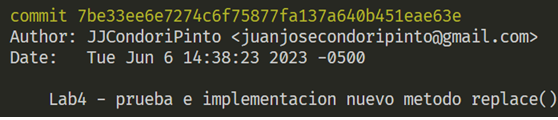
\includegraphics[width=5.85051in,height=1.21677in]{media/image33.png}

Commit de prueba e implementación de método replace()

\begin{quote}
Ejercicios:
\end{quote}

\begin{itemize}
\item
  Para resolver los siguientes ejercicios s´olo est´a permitido usar
  ciclos, condicionales, definici´on de listas por comprensi´on,
  sublistas, map, join, (+), lambda, zip, append, pop, range.
\item
  Implemente los m´etodos de la clase Picture. Se recomienda que
  implemente la clase picture por etapas, probando realizar los dibujos
  que se muestran en la siguiente preguntas.
\item
  Usando u´nicamente los m´etodos de los objetos de la clase Picture
  dibuje las siguientes figuras (invoque a draw)
\end{itemize}

Ejercicio a:

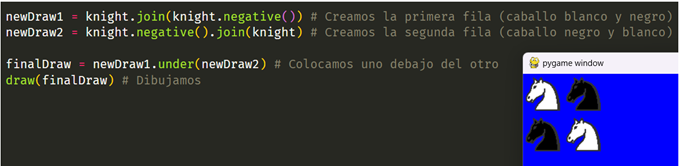
\includegraphics[width=7.08333in,height=1.73194in]{media/image34.png}

Para este ejercicio se consideraron los métodos join y negative, el
primero se utilizó para unir al lado derecho a las figuras contrarias,
es decir, caballos blanco -- negro y negro -- blanco, luego de ello se
colocó la nueva fila debajo de la otra, por último se imprimió la figura
final.

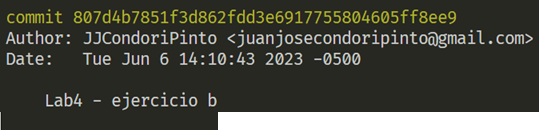
\includegraphics[width=5.61715in,height=1.16677in]{media/image35.png}

Ejercicio b:

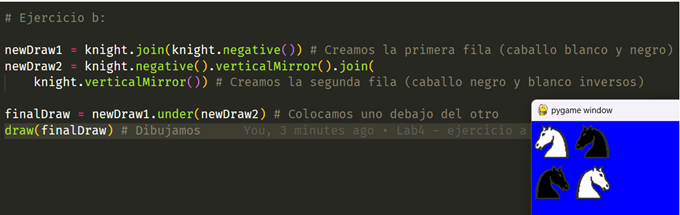
\includegraphics[width=7.08333in,height=2.23819in]{media/image36.png}

En este ejercicio se siguen los mismos pasos que en el anterior
ejercicio, con la diferencia de que para la segunda línea se obtiene la
figura general invertida, lo cual, retornará a los dos caballos
invertidos.

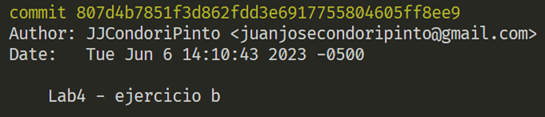
\includegraphics[width=5.67549in,height=1.21677in]{media/image37.png}

Ejercicio c:

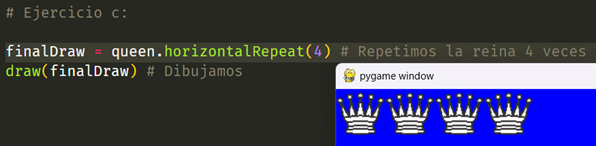
\includegraphics[width=6.20833in,height=1.52348in]{media/image38.png}

Para este ejercicios solo fue necesario el método horizontalRepeat(), ya
que la reina se repite 4 veces, uno al costado del otro.

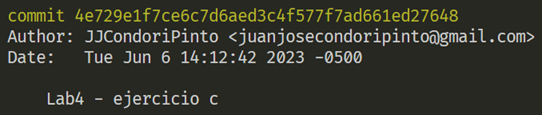
\includegraphics[width=5.65049in,height=1.2001in]{media/image39.png}

Ejercicio d:

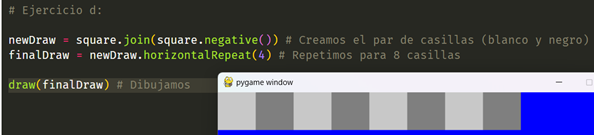
\includegraphics[width=6.18423in,height=1.40967in]{media/image40.png}

Este método hace uso de un patrón: casilla blanca junto con casilla
negra, el par repetido 4 veces para así formar una fila de 8.

Ejercicio e:

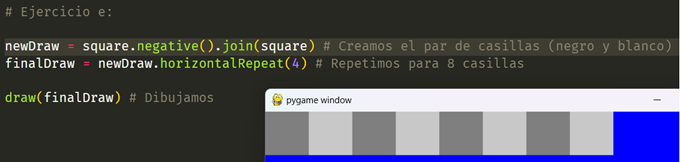
\includegraphics[width=7.08333in,height=1.69028in]{media/image41.png}

Misma lógica que en el anterior ejercicio, pero ahora el patrón es
inverso, vasta solo con unir primero la casilla negra y luego la blanca.

Ejercicio f:

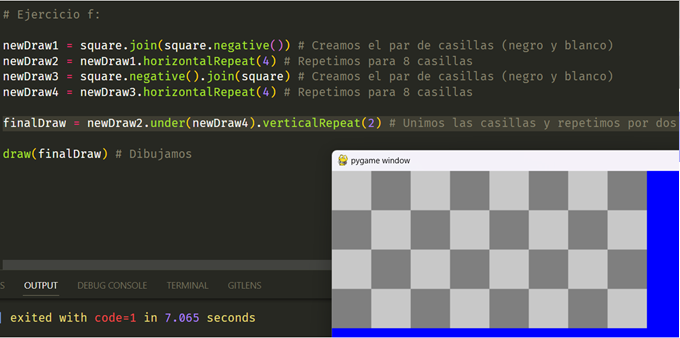
\includegraphics[width=7.07153in,height=3.52361in]{media/image42.png}

Para este ejercicio se toman los dos patrones anteriores, es decir, las
filas de 8 casillas intercaladas, una que inicia con blanca y otra con
negra, dichas filas se juntan una debajo de la otra y se duplica
verticalmente.

Ejercicio g:

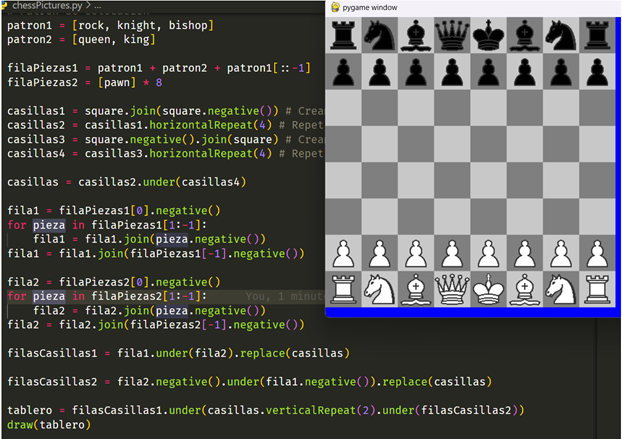
\includegraphics[width=6.47858in,height=4.57143in]{media/image43.png}

Este ejercicio resultó ser algo largo, primeramente, se crea un patrón
para las filas de piezas menores, reina y rey, primero obtenemos dicha
fila de piezas blancas y la unimos con una fila de 8 peones, luego de
ello los insertamos sobre un tablero parcial de 16 casillas, para ello
reciclamos el anterior ejercicio, repetimos con las piezas blancas y
separamos ambos bandos con un espacio de 32 casillas.

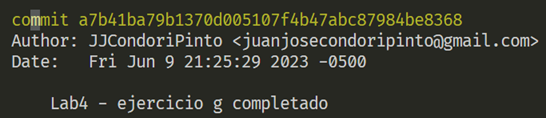
\includegraphics[width=5.69216in,height=1.22511in]{media/image44.png}

Commit de ejercicio g completado.

\begin{quote}
\textbf{Pregunta:} Explique: ¿Para qu´e sirve el directorio pycache?
\end{quote}

El directorio "pycache" es utilizado por el intérprete de Python para
almacenar archivos de caché generados automáticamente. Estos archivos de
caché tienen la extensión ".pyc" (bytecode compilado) y se crean cuando
se importan módulos en un programa de Python.

El propósito principal de la carpeta "pycache" y los archivos de caché
es mejorar el rendimiento al evitar la necesidad de recompilar los
archivos de código fuente de Python cada vez que se ejecuta un programa.
Cuando un módulo se importa, el intérprete de Python compila el código
fuente en bytecode y lo almacena en un archivo ".pyc". En las
ejecuciones posteriores, si el archivo ".pyc" existe y tiene una marca
de tiempo actualizada con respecto al archivo de código fuente original,
el intérprete de Python utiliza el bytecode almacenado en lugar de
recompilar el código fuente.

\begin{quote}
Tabla 1: Niveles de desempen˜o

Nivel
\end{quote}

\begin{longtable}[]{@{}
  >{\raggedright\arraybackslash}p{(\columnwidth - 8\tabcolsep) * \real{0.1132}}
  >{\raggedright\arraybackslash}p{(\columnwidth - 8\tabcolsep) * \real{0.2334}}
  >{\raggedright\arraybackslash}p{(\columnwidth - 8\tabcolsep) * \real{0.2040}}
  >{\raggedright\arraybackslash}p{(\columnwidth - 8\tabcolsep) * \real{0.2153}}
  >{\raggedright\arraybackslash}p{(\columnwidth - 8\tabcolsep) * \real{0.2340}}@{}}
\toprule
\begin{minipage}[b]{\linewidth}\raggedright
\begin{quote}
\textbf{Puntos}
\end{quote}
\end{minipage} & \begin{minipage}[b]{\linewidth}\raggedright
\begin{quote}
Insatisfactorio 25 \%
\end{quote}
\end{minipage} & \begin{minipage}[b]{\linewidth}\raggedright
\begin{quote}
En Proceso 50 \%
\end{quote}
\end{minipage} & \begin{minipage}[b]{\linewidth}\raggedright
\begin{quote}
Satisfactorio 75 \%
\end{quote}
\end{minipage} & \begin{minipage}[b]{\linewidth}\raggedright
\begin{quote}
Sobresaliente 100 \%
\end{quote}
\end{minipage} \\
\midrule
\endhead
\begin{minipage}[t]{\linewidth}\raggedright
\begin{quote}
\textbf{2.0}
\end{quote}
\end{minipage} & \begin{minipage}[t]{\linewidth}\raggedright
\begin{quote}
0.5
\end{quote}
\end{minipage} & \begin{minipage}[t]{\linewidth}\raggedright
\begin{quote}
1.0
\end{quote}
\end{minipage} & \begin{minipage}[t]{\linewidth}\raggedright
\begin{quote}
1.5
\end{quote}
\end{minipage} & \begin{minipage}[t]{\linewidth}\raggedright
\begin{quote}
2.0
\end{quote}
\end{minipage} \\
\begin{minipage}[t]{\linewidth}\raggedright
\begin{quote}
\textbf{4.0}
\end{quote}
\end{minipage} & \begin{minipage}[t]{\linewidth}\raggedright
\begin{quote}
1.0
\end{quote}
\end{minipage} & \begin{minipage}[t]{\linewidth}\raggedright
\begin{quote}
2.0
\end{quote}
\end{minipage} & \begin{minipage}[t]{\linewidth}\raggedright
\begin{quote}
3.0
\end{quote}
\end{minipage} & \begin{minipage}[t]{\linewidth}\raggedright
\begin{quote}
4.0
\end{quote}
\end{minipage} \\
\bottomrule
\end{longtable}

\begin{quote}
Tabla 3: Ru´brica para contenido del Informe y demostraci´on
\end{quote}

\begin{longtable}[]{@{}
  >{\raggedright\arraybackslash}p{(\columnwidth - 10\tabcolsep) * \real{0.1804}}
  >{\raggedright\arraybackslash}p{(\columnwidth - 10\tabcolsep) * \real{0.4334}}
  >{\raggedright\arraybackslash}p{(\columnwidth - 10\tabcolsep) * \real{0.0981}}
  >{\raggedright\arraybackslash}p{(\columnwidth - 10\tabcolsep) * \real{0.0922}}
  >{\raggedright\arraybackslash}p{(\columnwidth - 10\tabcolsep) * \real{0.1098}}
  >{\raggedright\arraybackslash}p{(\columnwidth - 10\tabcolsep) * \real{0.0862}}@{}}
\toprule
\multicolumn{2}{l}{\begin{minipage}[b]{\linewidth}\raggedright
\begin{quote}
Contenido y demostraci´on
\end{quote}
\end{minipage}} & \begin{minipage}[b]{\linewidth}\raggedright
\begin{quote}
Puntos
\end{quote}
\end{minipage} & \begin{minipage}[b]{\linewidth}\raggedright
\begin{quote}
Checklist
\end{quote}
\end{minipage} & \begin{minipage}[b]{\linewidth}\raggedright
\begin{quote}
Estudiante
\end{quote}
\end{minipage} & \begin{minipage}[b]{\linewidth}\raggedright
\begin{quote}
Profesor
\end{quote}
\end{minipage} \\
\midrule
\endhead
\begin{minipage}[t]{\linewidth}\raggedright
\begin{quote}
\textbf{1. GitHub}
\end{quote}
\end{minipage} & \begin{minipage}[t]{\linewidth}\raggedright
\begin{quote}
Hay enlace URL activo del directorio para el laboratorio hacia su
repositorio GitHub con c´odigo fuente terminado y f´acil de revisar.
\end{quote}
\end{minipage} & \begin{minipage}[t]{\linewidth}\raggedright
\begin{quote}
2
\end{quote}
\end{minipage} & X & 2 & \\
\begin{minipage}[t]{\linewidth}\raggedright
\begin{quote}
\textbf{2. Commits}
\end{quote}
\end{minipage} & \begin{minipage}[t]{\linewidth}\raggedright
\begin{quote}
Hay capturas de pantalla de los commits m´as importantes con sus
explicaciones detalladas. (El profesor puede preguntar para refrendar
calificaci´on).
\end{quote}
\end{minipage} & \begin{minipage}[t]{\linewidth}\raggedright
\begin{quote}
4
\end{quote}
\end{minipage} & X & 3 & \\
\begin{minipage}[t]{\linewidth}\raggedright
\begin{quote}
\textbf{3. C´odigo fuen- te}
\end{quote}
\end{minipage} & \begin{minipage}[t]{\linewidth}\raggedright
\begin{quote}
Hay porciones de c´odigo fuente importantes con numeraci´on y
explicaciones detalladas de sus funciones.
\end{quote}
\end{minipage} & \begin{minipage}[t]{\linewidth}\raggedright
\begin{quote}
2
\end{quote}
\end{minipage} & X & 2 & \\
\begin{minipage}[t]{\linewidth}\raggedright
\begin{quote}
\textbf{4. Ejecuci´on}
\end{quote}
\end{minipage} & \begin{minipage}[t]{\linewidth}\raggedright
\begin{quote}
Se incluyen ejecuciones/pruebas del c´odigo fuente explicadas
gradualmente.
\end{quote}
\end{minipage} & \begin{minipage}[t]{\linewidth}\raggedright
\begin{quote}
2
\end{quote}
\end{minipage} & \textbf{X} & 1.5 & \\
\begin{minipage}[t]{\linewidth}\raggedright
\begin{quote}
\textbf{5. Pregunta}
\end{quote}
\end{minipage} & \begin{minipage}[t]{\linewidth}\raggedright
\begin{quote}
Se responde con completitud a la pregunta for- mulada en la tarea. (El
profesor puede pregun- tar para refrendar calificaci´on).
\end{quote}
\end{minipage} & \begin{minipage}[t]{\linewidth}\raggedright
\begin{quote}
2
\end{quote}
\end{minipage} & X & 2 & \\
\begin{minipage}[t]{\linewidth}\raggedright
\begin{quote}
\textbf{6. Fechas}
\end{quote}
\end{minipage} & \begin{minipage}[t]{\linewidth}\raggedright
\begin{quote}
Las fechas de modificaci´on del c´odigo fuente stán dentro de los plazos
de fecha de entrega establecidos.
\end{quote}
\end{minipage} & \begin{minipage}[t]{\linewidth}\raggedright
\begin{quote}
2
\end{quote}
\end{minipage} & X & 1 & \\
\begin{minipage}[t]{\linewidth}\raggedright
\begin{quote}
\textbf{7. Ortograf´ıa}
\end{quote}
\end{minipage} & \begin{minipage}[t]{\linewidth}\raggedright
\begin{quote}
El documento no muestra errores ortogr´aficos.
\end{quote}
\end{minipage} & \begin{minipage}[t]{\linewidth}\raggedright
\begin{quote}
2
\end{quote}
\end{minipage} & X & 2 & \\
\begin{minipage}[t]{\linewidth}\raggedright
\begin{quote}
\textbf{8. Madurez}
\end{quote}
\end{minipage} & \begin{minipage}[t]{\linewidth}\raggedright
\begin{quote}
El Informe muestra de manera general una evoluci´on de la madurez del
c´odigo fuente, ex plicaciones puntuales pero precisas y un aca- bado
impecable. (El profesor puede preguntar para refrendar calificaci´on).
\end{quote}
\end{minipage} & \begin{minipage}[t]{\linewidth}\raggedright
\begin{quote}
4
\end{quote}
\end{minipage} & X & 3 & \\
\multicolumn{2}{l}{\begin{minipage}[t]{\linewidth}\raggedright
\begin{quote}
\textbf{Total}
\end{quote}
\end{minipage}} & \begin{minipage}[t]{\linewidth}\raggedright
\begin{quote}
20
\end{quote}
\end{minipage} & & 16.5 & \\
\bottomrule
\end{longtable}

\hypertarget{referencias}{%
\section{Referencias}\label{referencias}}

\begin{quote}
\url{https://www.w3schools.com/python/python_reference.asp}
\url{https://docs.python.org/3/tutorial/}´
\end{quote}

\end{document}
